

\tikzset{every picture/.style={line width=0.75pt}} %set default line width to 0.75pt        

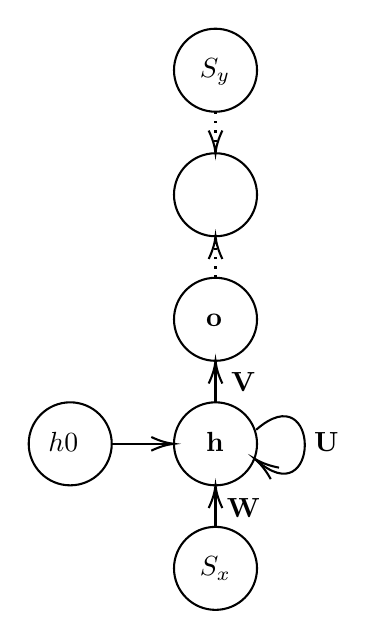
\begin{tikzpicture}[x=0.75pt,y=0.75pt,yscale=-1,xscale=1]
%uncomment if require: \path (0,350); %set diagram left start at 0, and has height of 350

%Shape: Circle [id:dp06377137847654812] 
\draw   (110,270) .. controls (110,258.95) and (118.95,250) .. (130,250) .. controls (141.05,250) and (150,258.95) .. (150,270) .. controls (150,281.05) and (141.05,290) .. (130,290) .. controls (118.95,290) and (110,281.05) .. (110,270) -- cycle ;
%Shape: Circle [id:dp3067158430514074] 
\draw   (110,210) .. controls (110,198.95) and (118.95,190) .. (130,190) .. controls (141.05,190) and (150,198.95) .. (150,210) .. controls (150,221.05) and (141.05,230) .. (130,230) .. controls (118.95,230) and (110,221.05) .. (110,210) -- cycle ;
%Shape: Circle [id:dp611977585123813] 
\draw   (110,150) .. controls (110,138.95) and (118.95,130) .. (130,130) .. controls (141.05,130) and (150,138.95) .. (150,150) .. controls (150,161.05) and (141.05,170) .. (130,170) .. controls (118.95,170) and (110,161.05) .. (110,150) -- cycle ;
%Shape: Circle [id:dp14694306376973554] 
\draw   (110,90) .. controls (110,78.95) and (118.95,70) .. (130,70) .. controls (141.05,70) and (150,78.95) .. (150,90) .. controls (150,101.05) and (141.05,110) .. (130,110) .. controls (118.95,110) and (110,101.05) .. (110,90) -- cycle ;
%Shape: Circle [id:dp5910587750622855] 
\draw   (110,30) .. controls (110,18.95) and (118.95,10) .. (130,10) .. controls (141.05,10) and (150,18.95) .. (150,30) .. controls (150,41.05) and (141.05,50) .. (130,50) .. controls (118.95,50) and (110,41.05) .. (110,30) -- cycle ;
%Straight Lines [id:da2011519740133465] 
\draw    (130,250) -- (130,232) ;
\draw [shift={(130,230)}, rotate = 450] [color={rgb, 255:red, 0; green, 0; blue, 0 }  ][line width=0.75]    (10.93,-3.29) .. controls (6.95,-1.4) and (3.31,-0.3) .. (0,0) .. controls (3.31,0.3) and (6.95,1.4) .. (10.93,3.29)   ;
%Straight Lines [id:da12556610154917158] 
\draw    (130,190) -- (130,172) ;
\draw [shift={(130,170)}, rotate = 450] [color={rgb, 255:red, 0; green, 0; blue, 0 }  ][line width=0.75]    (10.93,-3.29) .. controls (6.95,-1.4) and (3.31,-0.3) .. (0,0) .. controls (3.31,0.3) and (6.95,1.4) .. (10.93,3.29)   ;
%Straight Lines [id:da2830637374783129] 
\draw  [dash pattern={on 0.84pt off 2.51pt}]  (130,130) -- (130,112) ;
\draw [shift={(130,110)}, rotate = 450] [color={rgb, 255:red, 0; green, 0; blue, 0 }  ][line width=0.75]    (10.93,-3.29) .. controls (6.95,-1.4) and (3.31,-0.3) .. (0,0) .. controls (3.31,0.3) and (6.95,1.4) .. (10.93,3.29)   ;
%Straight Lines [id:da15964377279739028] 
\draw  [dash pattern={on 0.84pt off 2.51pt}]  (130,50) -- (130,68) ;
\draw [shift={(130,70)}, rotate = 270] [color={rgb, 255:red, 0; green, 0; blue, 0 }  ][line width=0.75]    (10.93,-3.29) .. controls (6.95,-1.4) and (3.31,-0.3) .. (0,0) .. controls (3.31,0.3) and (6.95,1.4) .. (10.93,3.29)   ;
%Curve Lines [id:da7776893016719004] 
\draw    (149.59,203.23) .. controls (180.96,175.68) and (180.8,245.86) .. (149.31,217.52) ;
\draw   (156.6,227) .. controls (154.52,223.15) and (151.98,219.92) .. (149,217.29) .. controls (152.42,219.3) and (156.29,220.69) .. (160.6,221.47) ;

%Shape: Circle [id:dp09339586372332742] 
\draw   (40,210) .. controls (40,198.95) and (48.95,190) .. (60,190) .. controls (71.05,190) and (80,198.95) .. (80,210) .. controls (80,221.05) and (71.05,230) .. (60,230) .. controls (48.95,230) and (40,221.05) .. (40,210) -- cycle ;
%Straight Lines [id:da909898274600083] 
\draw    (80,210) -- (108,210) ;
\draw [shift={(110,210)}, rotate = 180] [color={rgb, 255:red, 0; green, 0; blue, 0 }  ][line width=0.75]    (10.93,-3.29) .. controls (6.95,-1.4) and (3.31,-0.3) .. (0,0) .. controls (3.31,0.3) and (6.95,1.4) .. (10.93,3.29)   ;

% Text Node
\draw (121,263) node [anchor=north west][inner sep=0.75pt]    {$S_\Vector{x}$};
% Text Node
\draw (48,203) node [anchor=north west][inner sep=0.75pt]    {$\Elem{h}{0}$};
% Text Node
\draw (124,203) node [anchor=north west][inner sep=0.75pt]    {$\mathbf{h}$};
% Text Node
\draw (124,146) node [anchor=north west][inner sep=0.75pt]    {$\mathbf{o}$};
% Text Node
\draw (123,82) node [anchor=north west][inner sep=0.75pt]    {$\Loss$};
% Text Node
\draw (121,23) node [anchor=north west][inner sep=0.75pt]    {$S_\Vector{y}$};
% Text Node
\draw (134,235) node [anchor=north west][inner sep=0.75pt]    {$\mathbf{W}$};
% Text Node
\draw (176,203) node [anchor=north west][inner sep=0.75pt]    {$\mathbf{U}$};
% Text Node
\draw (136,174) node [anchor=north west][inner sep=0.75pt]    {$\mathbf{V}$};


\end{tikzpicture} 